\chapter{معیارهای جهش و فرآیند}
 
\label{chap:method}
با  مطالعات مروری انجام شده نقاطی از این حوزه که نیازمند پژوهش بیشتر هستند تا بتوان به وسیله‌ی آن به ارائه‌ی روشی کاراتر در پیش‌بینی خطا پرداخت مشخص شد. مقاله‌ی \cite{bowes2016mutation} اولین مقاله‌ای است که  یک  روش پیش‌بینی خطا با استفاده از تحلیل جهش ارائه نموده  است و این موضوع نیازمند تحقیق بیشتر است. از طرف دیگر بر طبق مقاله‌ی \cite{radjenovic2013software} استفاده از معیارهای فرآیند علی‌رغم توانایی بالقوه‌ای که در پیش‌بینی خطا دارند، در پژوهش‌های کمتری مورد بررسی قرار گرفته‌اند. یکی از دلایل آن می‌تواند نو ظهور بودن این معیارها نسبت به سایرین باشد. معیارهای فرآیند از جنبه‌های مختلف نیز از سایر معیار‌ها برتری دارند \cite{rahman2013and}. \\
این پایانامه قصد دارد سه رویکرد  پیشنهادی را به منظور بهبود پیش‌بینی خطا بررسی کند.  این رویکردها عبارتند از:
\begin{enumerate}
\item
معیارهای جهش و معیارهای فرآیند در کنار یکدیگر استفاده می‌شوند و به وسیله‌ی آنها پیش‌بینی انجام می گیرد. این دو دسته معیار در پژوهش‌های گذشته مطرح شده‌اند اما تاکنون در کنار یکدیگر قرار نگرفته‌اند.
\item
معیارهای جدیدی مطرح می‌شوند که مبتنی بر مفاهیم آزمون جهش و فرآیند توسعه‌ی نرم‌افزار است.
\item
معیارهای جدیدی مطرح می‌شوند که با کمک مفاهیم جهش سعی در بهبود معیارهای فرآیند دارند.
\end{enumerate}

همچنین جهت استخراج معیارها و انجام پیش‌بینی خطا در این پایانامه ابزاری به نام JPredict طراحی و ساخته می‌گردد. جهت مشخص‌تر شدن نحوه‌ی قرارگیری معیارهای مطح شده نمودار ون معیارهای پیش‌بینی خطا در شکل \ref{fig:venn} نمایش داده شده است. 

\begin{figure}[H]
	\centering
	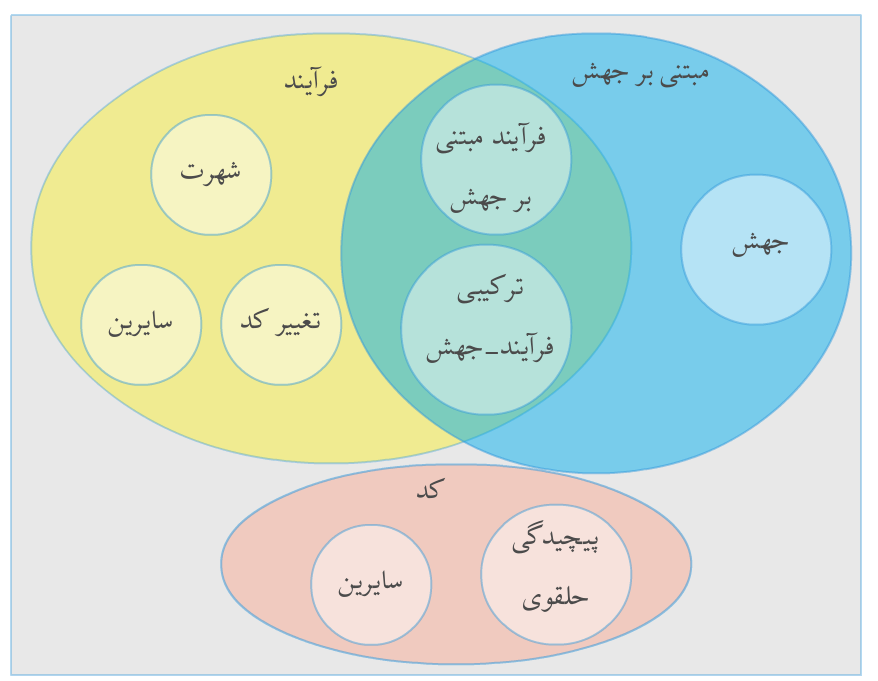
\includegraphics[width=.7\textwidth]{img/method/venn.png}
	\caption{نمودار ون معیارهای پیش‌بینی خطا }
	\label{fig:venn}
\end{figure}


\section{معیارهای جهش و فرآیند}
\label{sec:method-phase1}

این رویکرد با توجه به مقاله‌ی \cite{bowes2016mutation} مطرح شده که در آن بررسی به کارگیری معیارهای جهش و فرآیند را در پژوهش‌های آتی توصیه می‌کند.  همچنین  معیار جهش یک معیار  مرتبط با کد است. مقاله‌ی \cite{rahman2013and}  بیان می‌کند که معیارهای کد ایستا هستند و تمایل دارند که یک موجودیت را در انتشارهای متوالی حاوی خطا معرفی کنند. حال شرایطی را در نظر بگیرید که که امتیاز جهش در یک موجودیت کم باشد و دلیل آن کافی نبودن مجموعه آزمون باشد چراکه توسعه‌دهندگان از درست بودن کد اطمینان دارند یا اینکه پس از انتشارهای متوالی خطاها بر طرف شده است. چنین موجودیتی حاوی خطا نیست اما با توجه به معیار جهش خطا‌خیز است. با در نظر گرفتن معیارهای فرآیند در مورد این موجودیت که نشان می‌دهند پایدار و بدون تغییر است از میزان خطا‌خیز بودن آن کاسته می‌شود و انتظار می‌رود کارایی مدل پیش‌بینی بهبود یابد. 
برای  انجام این رویکرد مجموعه معیارهای جهش  از پژوهش \cite{bowes2016mutation}  و معیارهای فرآیند از پژوهش \cite{rahman2013and} انتخاب می‌شوند. در جداول  \ref{tab:process-metircs} و \ref{tab:mutation-metircs} معیارهای مورد نظر آورده شده است و به ترتیب در قسمت‌های \ref{subsec:metrics} و \ref{sec:mutation} معرفی شده‌اند.\\


از آنجا که  در این پایانامه پیش‌بینی‌ها در سطح پرونده انجام می‌شود، معیارها برای هر پرونده جداگانه محاسبه می‌شوند. در ادامه هر یک از معیارهای فرآیند معرفی و نحوه‌ی محاسبه‌ی آن‌ها بیان می‌شود. معیارهای جهش به طور مستقیم توسط ابزارهای موجود محاسبه‌ می‌گردد و نیازمند توضیح بیشتر نیستند.\\




%%%%%%%%%%%
\section{معیارهای جهش مبتنی بر فرآیند}
\label{sec:method-phase-two}
در رویکرد دوم، چهار معیار جدید در این پایانامه معرفی می‌شوند که با استفاده از مفاهیم آزمون جهش و تاریخچه‌ی توسعه‌ی نرم‌افزار ساخته می‌شوند. از این رو این معیارها  \نام{معیارهای جهش مبتنی بر فرآیند}{Process Based Mutation Metrics (PBMM)} نامیده شده‌اند.

\begin{table}[H] 
	\renewcommand*{\arraystretch}{1.7}	
	\centering
	 \caption{نمادهای استفاده شده در تعاریف معیارها  }
	\label{tab:metric-symbols}
	\newcolumntype{C}{>{\centering\arraybackslash} m } 
	\begin{tabular}{ |c|c|}
		
		\hline
		\hline
		نماد  & توضیح
		\\
		\hline
		\hline
\lr{$Mutants(c,f)$} & 
مجموعه‌ی جهش‌یافته‌های پرونده‌ی f در ثبت یا انتشار c
		\\
		\hline
	$C_i$ &
	ثبت شماره‌ی i
	\\
	\hline
	$R_i$ & انتشار شماره‌ی i	
	\\
	\hline

$C(R)$ & ثبت متعلق به انتشار R	
\\
\hline	
$Seq(C)$ & شماره‌ی ثبت C	
\\
\hline

$LR(i)$ & آخرین انتشار ماقبل ثبت شماره‌ی i
	\\
	\hline
	$MuScore(c,f)$ & امتیاز جهش پرونده‌ی f در ثبت یا انتشار c
	\\
	\hline
 $\delta^+(x)$ & 
 $
 \begin{cases}
 x      & \quad x > 0 \text{اگر } \\
 0 & \quad  x <= 0 \text{ اگر}
 \end{cases}
$
 \\
 \hline
  $\delta^-(x)$ & 
 $
 \begin{cases}
 0      & \quad x > 0 \text{اگر } \\
 x & \quad  x <= 0 \text{ اگر}
 \end{cases}
 $
 \\
 \hline
		
	\end{tabular}
\end{table}

\begin{table}[H] 
	\renewcommand*{\arraystretch}{1.5}	
	\centering
	\caption{عملگرهای استفاده شده در مثال‌ها}
	\label{tab:example-mutators}
	\newcolumntype{C}{>{\centering\arraybackslash} m } 
	\begin{tabular}{ |c|c|c|}
		
		\hline
		\hline
		عملگر  & نسخه‌ی اصلی & نسخه‌ی جهش‌یافته
		\\
		\hline
		\hline
	
\lr{Arithmetic Operator Replacement} &
a + b & a - b 
		\\
		\hline
	\lr{Arithmetic Operator Replacement} &
	a - b & a + b 	\\
	\hline
		\lr{Arithmetic Operator Replacement} &
	a * b & a / b 	\\
	\hline
	\lr{Arithmetic Operator Replacement} &
	a \% b & a / b 	\\
	\hline
	\lr{Expression Value Replacement} & \lr{int a = x} & \lr{int a = 0} \\
	\hline
\lr{	Relational Operator Replacemen} & a < b & a > b \\
	\hline
	\lr{	Relational Operator Replacemen} & a < b & a <= b \\
	\hline
			
	\end{tabular}
\end{table}

 

\begin{enumerate}
	\item  
	\textbf{
		تعداد جهش‌یافته‌های تولید شده‌ی جدید نسبت به انتشار قبلی برنامه: }همانطور که در مقاله‌ی \cite{just2014mutants} مطرح شده جهش‌یافته‌ها جایگزین خوبی برای خطاهای واقعی می‌باشند. زمانی که تعداد جهش‌یافته‌های جدید زیاد باشد یعنی تغییراتی که خطا‌خیز‌تر هستند بیشتر است. به منظور محاسبه‌ی این معیار لازم است خطوط اضافه شده به پرونده‌ی مورد نظر در ثبت کنونی، نسبت به انتشار قبلی مشخص شود و سپس تعداد جهش یافته‌هایی که این خطوط تولید می‌کنند شمرده شوند. این معیار در فرمول زیر خلاصه می‌شود. \\
	
\begin{latin}

$NewMutants(C_i,f) = || Mutants(C_i,f) - Mutants(LR(i),f)||$

\end{latin}

	
\textbf{مثال اول} : 
در شکل \ref{fig:example1} مثالی  از روند توسعه پرونده‌ی در طول یک انتشار آورده شده است. قسمت چپ این شکل نشان می‌دهد که پرونده‌ی Calculator در انتشار ۲.۳ دارای دو تابع جمع و تفریق بوده است. ثبت مربوط به انتشار ۲.۳،  شماره‌ی دنباله‌ی ۱۵۲۲ را دارد یعنی از ابتدای پروژه تا این ثبت ۱۵۲۲ ثبت دیگر انجام گرفته است. با استفاده از CommitID نیز می‌توان این ثبت را از سامانه‌ی کنترل نسخه فراخوانی کرد. معیار توضیح داده شده در بالا را می‌خواهیم برای  پرونده‌ی  Calculator در ثبت نشان داده شد در قسمت راست شکل محاسبه کنیم. این شکل نشان می‌دهد که پروژه از انتشار قبلی تا ثبت مورد نظر 51 ثبت دیگر داشته و در میان این آنها در دو ثبت پرونده‌ی Calculator تغییر کرده است. 
 همانور که در شکل مشخص است برای محاسبه‌ی معیار تنها لازم است که ثبت مورد نظر و ثبت مربوط به آخرین انتشار در نظر گرفته شود. تعداد جهش‌یافته‌هایی که از هر خط تولید می‌شود در کنار آنها نوشته شده است. عملگرهای استفاده شده جهت تولید جهش یافته در جدول  \ref{tab:example-mutators} آمده است. در این مثال خطوط ۱۱ تا ۱۷ به پرونده اضافه شده است. از این خطوط می‌توان ۶ جهش یافته تولید کرد و در نهایت تعداد جهش‌یافته‌های جدید نسبت به انتشار قبلی برابر ۶ می‌شود. 

\begin{figure}[H]
	\centering
	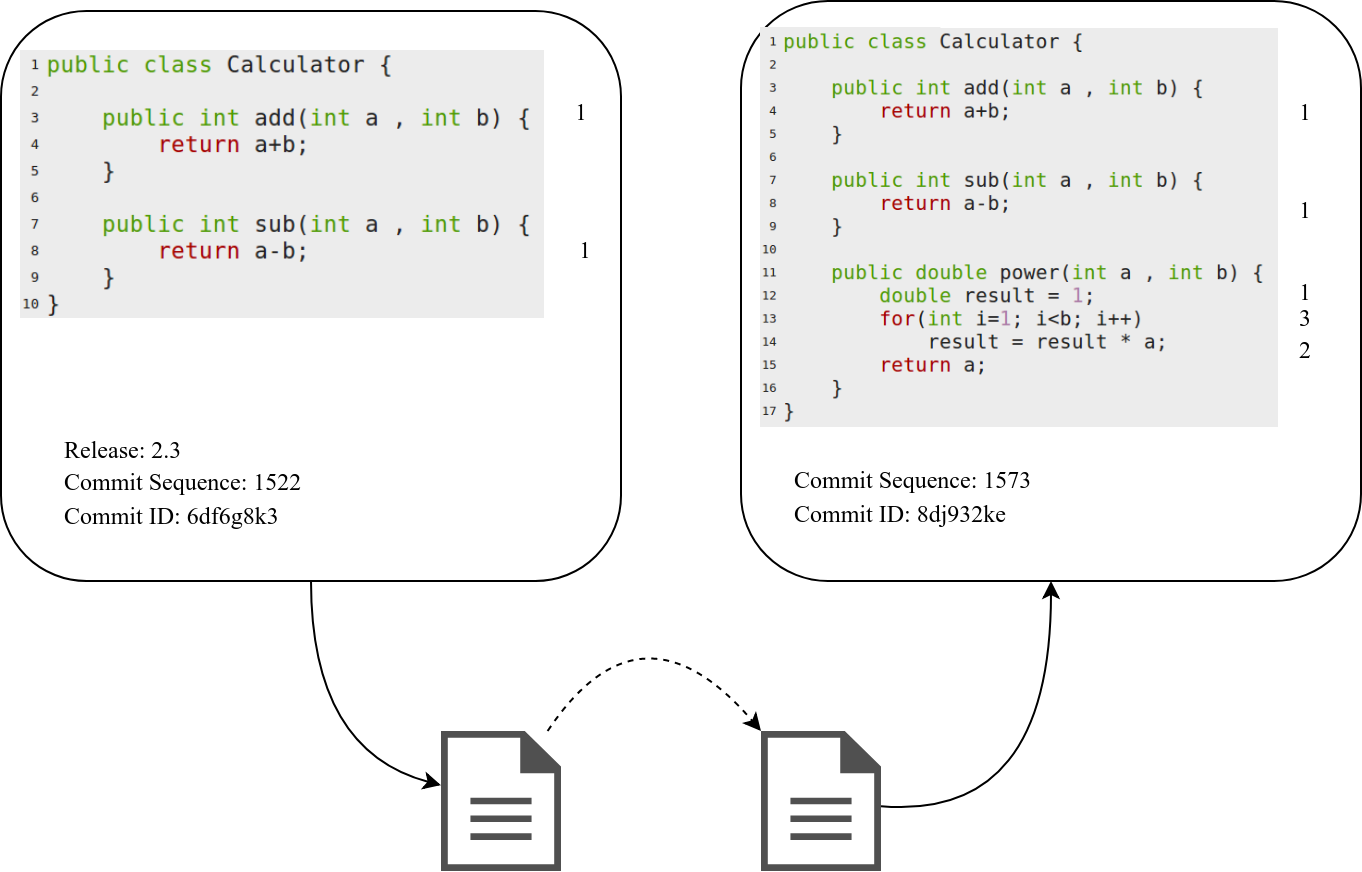
\includegraphics[width=1\textwidth]{img/method/example1.png}
	\caption{ تاریخچه‌ی پرونده‌یCalculator در مثال اول}
	\label{fig:example1}
\end{figure}



\item 
\textbf{
		تعداد جهش‌یافته‌های متمایز در چند انتشار اخیر:} این معیار نشان می‌دهد موجودیت مورد بررسی به چه میزان سابقه‌ی تغییراتی را دارد که احتمال بروز خطا را افزایش می‌دهد. تعداد انتشارها باید به گونه‌ای باشد که کم یا زیاد نباشد. زیرا تعداد انتشارهای کم سبب می‌شود تفاوت چندانی با معیار قبلی نداشته باشد و سابقه‌ی تغییرات به اندازه‌ی کافی مد نظر قرار نگیرد. از طرف دیگر در نظر گرفتن تعداد زیادی انتشار، هم هزینه‌بر است و هم به دلیل تغییرات زیاد  پرونده در طول توسعه‌ی نرم‌افزار اطلاعات اولیه مفید نخواهد بود.  تعداد انتشارهای  در نظر گرفته شده در این پایانامه چهار می‌باشد. نحوه‌ی محاسبه به این شکل است که برای هر انتشار تعداد جهش‌یافته‌ها در انتشار جدید، نسبت به قبلی  شمرده می‌شود و با یکدیگر جمع زده  می‌شوند. این معیار در فرمول زیر خلاصه می‌شود. 
	

\begin{latin}
\[ 	
DistinctMutant(C_i,f) = \mathlarger{\sum}\limits_{j=LR(c_i)-3}^{LR(c_i)} 
|| Mutants(R_{j+1},f) - Mutants(R_j,f)|| 
\]
\end{latin}

	
\textbf{مثال دوم:}
در شکل \ref{fig:example2} روند توسعه‌ی پرونده‌ی  Calculator از انتشار ۱ تا ۲.۳ نشان داده شده است. مشابه مثال قبل تعداد جهش‌یافته‌هایی که از هر خط توسط عملگرهای جدول \ref{tab:example-mutators}  تولید می‌شود در کنار آن نوشته شده است. در این مثال قصد داریم معیار مطرح شده را برای پرونده‌ی Calculator‌ در ثبت با شماره‌ی ۱۵۷۳ استخراج کنیم. انتشارهای‌ ما قبل از این ثبت در شکل  \ref{fig:example2} نشان داده شده است. در انتشار دوم یک تابع اضافه شده که یک جهش یافته می‌توان در آن ایجاد کرد. در انتشار سوم تابع mode حذف شده  تابع sub جایگزین آن شده است. در تابع جایگزین هم یک جهش یافته می‌توان استخراج کرد. در نهایت تعداد جهش یافته‌های متمایز در انتشارهای ما قبل برابر ۳ خواهد بود. 


\begin{figure}[H]
	\centering
	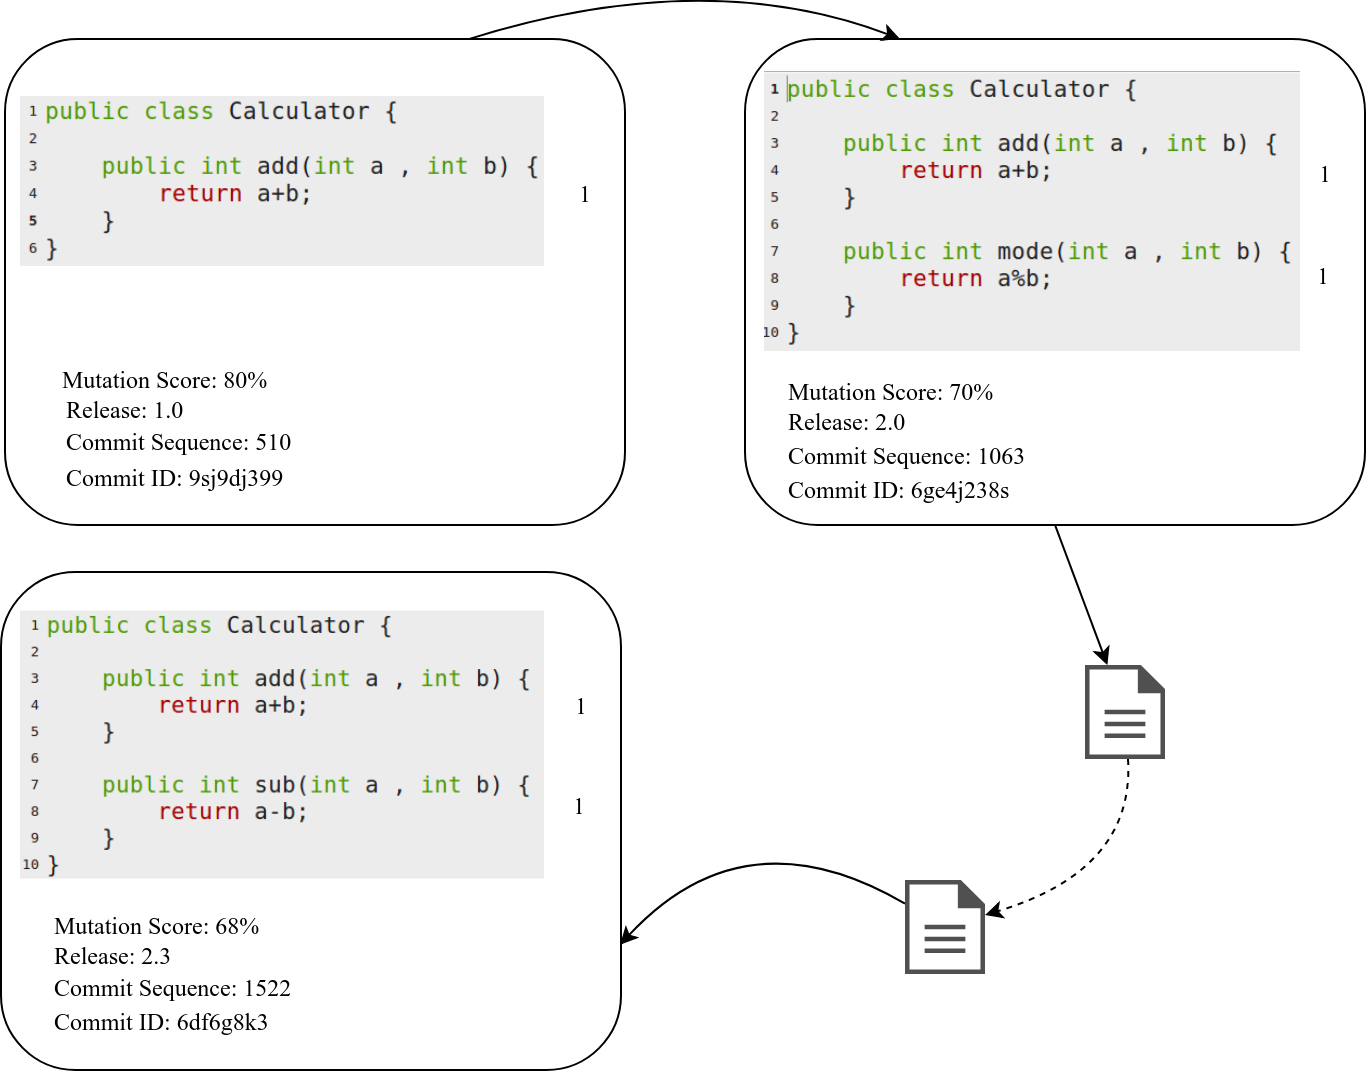
\includegraphics[width=1\textwidth]{img/method/example2.png}
	\caption{ تاریخچه‌ی پرونده‌یCalculator در مثال دوم و سوم}
	\label{fig:example2}
\end{figure}

	\item 
	\textbf{
		میزان تغییرات مثبت امتیاز جهش  در چند انتشار اخیر:}
	تغییرات امتیاز جهش نشان از تغییرات در برنامه و آزمون‌های نرم‌افزار است. این معیار نشان می‌دهد این تغییرات به چه میزان در جهت بهبود کیفیت نرم‌افزار بوده. چراکه امتیاز بالاتر جهش نشان از کیفیت بهتر آزمون‌ها و در نتیجه نرم‌افزار است.  به منظور محاسبه‌ی این معیار در هر انتشار امتیاز جهش محاسبه می‌شود و در صورتی که نسبت به انتشار قبلی تغییر مثبت  بود به مجموع تغییرات  مثبت  افزوده می‌شود. این معیار در فرمول زیر خلاصه شده است.
\begin{latin}
\[
PositiveChanges(C_i,f) = \mathlarger{\sum}\limits_{j=LR(c_i)-3}^{LR(c_i)} 
\mathlarger{\delta}^+\bigg(MuScore(R_{j+1},f) - MuScore(R_j,f)\bigg) 
\]
\end{latin}	


	\item 
	\textbf{
		میزان تغییرات منفی امتیاز جهش در چند انتشار اخیر:}
	این معیار مشابه معیار سوم عمل می‌کند با این تفاوت که میزان تغییرات در خلاف جهت بهبود نرم‌افزار را می‌سنجد. این معیار در فرمول زیر خلاصه شده است.
\begin{latin}
	\[
	NegetiveChanges(C_i,f) = \mathlarger{\sum}\limits_{j=LR(c_i)-3}^{LR(c_i)} 
	\mathlarger{\delta}^-\bigg(MuScore(R_{j+1},f) - MuScore(R_j,f)\bigg) 
	\]
\end{latin}	
\textbf{مثال سوم:}
در این مثال تغییرات مثبت و منفی امتیاز جهش در انتشارهای قبل محاسبه می‌شود. برای این منظور روند توسعه‌ی پرونده‌ی Calculator در شکل \ref{fig:example2}  در نظر گرفته می‌شود. امتیاز جهش از انتشار اول به دوم ۱۰ درصد کاهش یافته و از انتشار دوم به سوم نیز دو درصد کاهش داشته است. در نتیجه مجموعه تغییرات مثبت صفر و مجموعه تغییرات منفی برابر ۱۲ و تغییرات مثبت صفر است. 
	
\end{enumerate}


\section{معیارهای ترکیبی جهش-فرآیند}
رویکرد سوم با توجه به مطالب گفته شده در مقاله‌ی \cite{rahman2013and} مطرح شده که بیان می‌کند معیارها هر چقدر هم که پویا باشند (دچار رکود نشوند، مانند معیارهای فرآیند) زمانی در پیش‌بینی خطا مفید هستند که همراه با ایجاد خطا باشند. نکته‌ی قابل توجه این است که همه‌ی تغییرات در یک پرونده به یک اندازه  بر پیچیدگی پرونده نمی‌افزایند و به عبارت دیگر موجب بروز خطا نمی‌شوند. به عنوان مثال در یک پرونده به زبان جاوا ممکن است \واژه{توضیح} و یا \واژه{مستند‌جاوا} وجود داشته باشد که بروزرسانی یا اضافه و کم شدن آنها تاثیری بر روند اجرای برنامه و میران پیچیدگی ندارند با این حال در محاسبه‌ی معیارهای پیش‌بینی خطا در نظر گرفته می‌شوند. هدف از ارائه‌ی معیارهای \نام{ترکیبی جهش-فرآیند}{Process-Mutation Hybrid} بهبود کاستی‌های معیارهای فرآیند در چنین شرایطی است. در اینجا دو معیار \موکد{مقدار نرمال شده‌ی خطوط اضافه شده} و یا \موکد{کم شده}  جهت اصلاح انتخاب شده‌اند.  این دو معیار جز شاخص‌ترین معیارهای فرآیند هستند.\\
در نگاه اول  این ایده به ذهن می‌رسد که با توجه به تعداد جهش‌یافته‌هایی که  اضافه   کردن  خط ایجاد می‌کند و یا حذف هر خط  از بین می‌برد. اضافه یا کم شدن خطوط وزن دهی شود و به منظور اجرای آن از دو  فرمول زیر بهره گرفت.\\
\begin{latin}
	
	$M_1 =\ number\ of\ lines\ added\ \times \ number\ of\ muatants\ derived$\\
	
	$M_2 =\ number\ of\ lines\ deleted\ \times \ number\ of\ mutants\ derived$\\
\end{latin}


با وجود مناسب بودن ایده ی اولیه با بررسی‌های بیشتر دو مشکل در معیارهای فوق مشخص می‌شود.\\
مشکل اول : هدف از ارئه ی این معیارها وزن دهی به خطوط اضافه و کم شده است. نکته قابل توجه این است که هر خط باید به صورت جداگانه وزن دهی شود و وزن یک خط بر وزن خط دیگر تأثیری نداشته باشد. مثال زیر را در نظر بگیرید.
\begin{latin}
\flushleft
//this method is important  \emph{→ 0 mutant} \\
// this method get root of \emph{→ 0 mutant}\\
// sum of a plus b \emph{→ 0 mutant} \\ 
b = sqrt(a+b) \emph{→ 2 mutant} \\
\end{latin}

فرض کنید ۴ خط بالا به یک پرونده اضافه شده است. معیار  \موکد{مقدار نرمال شده‌ي خطوط اضافه شده} قبل از نرمال سازی عدد چهار را نمایش می‌دهد در حالی که از این چهار خط ۳ خط توضیح است. حال معیار اولیه پیشنهادی برابر ۸ خواهد بود که بدیهی است، از هدف ارايه ی معیار فاصله گرفته است. حال اگر تنها جهش یافته‌های تولید شده در خطوط اضافه شده را در نظر بگیریم این مقدار می‌تواند جایگزین مناسبی باشد. در‌ واقع نگاشتی  ارائه می‌شود که هر خط از برنامه را به یک عدد نگاشت می‌دهد. این عدد میزان پیچیدگی آن خط و یا احتمال بروز خطا را تعریف می‌کند.  لازم به یادآوری است که در مقاله‌ی  \cite{just2014mutants} اشاره شده که جهش یافته ها جایگزین خوبی برای خطاهای واقعی هستند. این نگاشت برابر است با تعداد جهش یافته های تولید شده در آن خط.

مشکل دوم: این معیار برای عملکرد هرچه بهتر مشابه معیار  \موکد{مقدار نرمال شده‌ی خطوط اضافه شده}‌ نیاز به نرمال‌سازی دارد. به جهت نرمال‌سازی نمی‌توان از همان روش استفاده کنیم چراکه در آن وزن‌دهی به خطوط وجود ندارد و از آن مهم‌تر توضیحات را نیز در نظر می‌گیرد. از طرف دیگر این امکان وجود ندارد که برای تمام خطوط اضافه یا کم شده در کل پروژه در طول یک انتشار جهش یافته تولید شود (به دلیل زمانبر بودن و پیچیدگی‌های فراوان در پیاده‌سازی). در مقاله‌ی \cite{bird2011don} اشاره شده که تعداد ثبت‌ها می‌تواند نشانگر میزان تغییرات باشد. بنابرین از تعداد ثبت‌های کل پروژه در طول یک انتشار به منظور نرمال‌سازی استفاده خواهد شد.\\

\begin{latin}
\begin{multline*}
NormalWeightedAddedLines(c_i,f) =\\ \frac{ \mathlarger{\sum}\limits_{j=Seq(C(LR(c_i)))}^{i} ||Mutants(C_j,f) - Mutants(C_{j-1,f})||
	}{i - Seq(C(LR(c_i)))}\\
\end{multline*}
\end{latin}

\begin{latin}
	\begin{multline*}
	NormalWeightedDeletedLines(c_i,f) =\\ \frac{ \mathlarger{\sum}\limits_{j=Seq(C(LR(c_i)))}^{i} ||Mutants(C_{j-i},f) - Mutants(C_j,f)||
	}{i - Seq(C(LR(c_i)))}\\
	\end{multline*}
\end{latin}

 
\textbf{مثال چهارم:}
در این مثال معیار‌های مقدار نرمال شده‌ی خطوط اضافه‌ی وزن دهی شده و خطوط حذف شده برای شکل \ref{fig:example3} محاسبه می‌شود. زمانی که قرار است برای پرونده‌ی Calculator  در ثبت ۱۵۷۳ معیارها محاسبه شود لازم است آخرین انتشار و ثبت‌های ماقبل بین انتشار و ثبت ۱۵۷۳ بررسی شوند. آخرین انتشار برای این ثبت انتشار ۲.۳ می‌باشد و  در این بین این پرونده تنها در ثبت شماره‌ی ۱۳۳۹ تغییر کرده است. \\
در ثبت 1568 خطوط ۱۱ تا ۱۶ نسبت به ثبت قبلی (انتشار ۲.۳) تغییر کرده است. از این خطوط تنها یک جهش‌یافته را می‌توان تولید کرد. در ثبت ۱۵۷۳ خطوط ۱۱ تا ۱۷ جایگزین شده‌اند که این خطوط می‌توانند ۶ جهش یافته را تولید کنند. تعداد کل ثبت‌های پروژه در این بازه  برابر نیز برابر ۵۱ 
(۱۵۲۲-۱۵۷۳) 
است. 
\begin{latin}
\[
NormalWeightedAddedLine = \frac{1+6}{51} = 0.137\]\\
\[
NormalWeightedDeletedLine = \frac{1}{51} = 0.019
\]
\end{latin}



\begin{figure}[H]
	\centering
	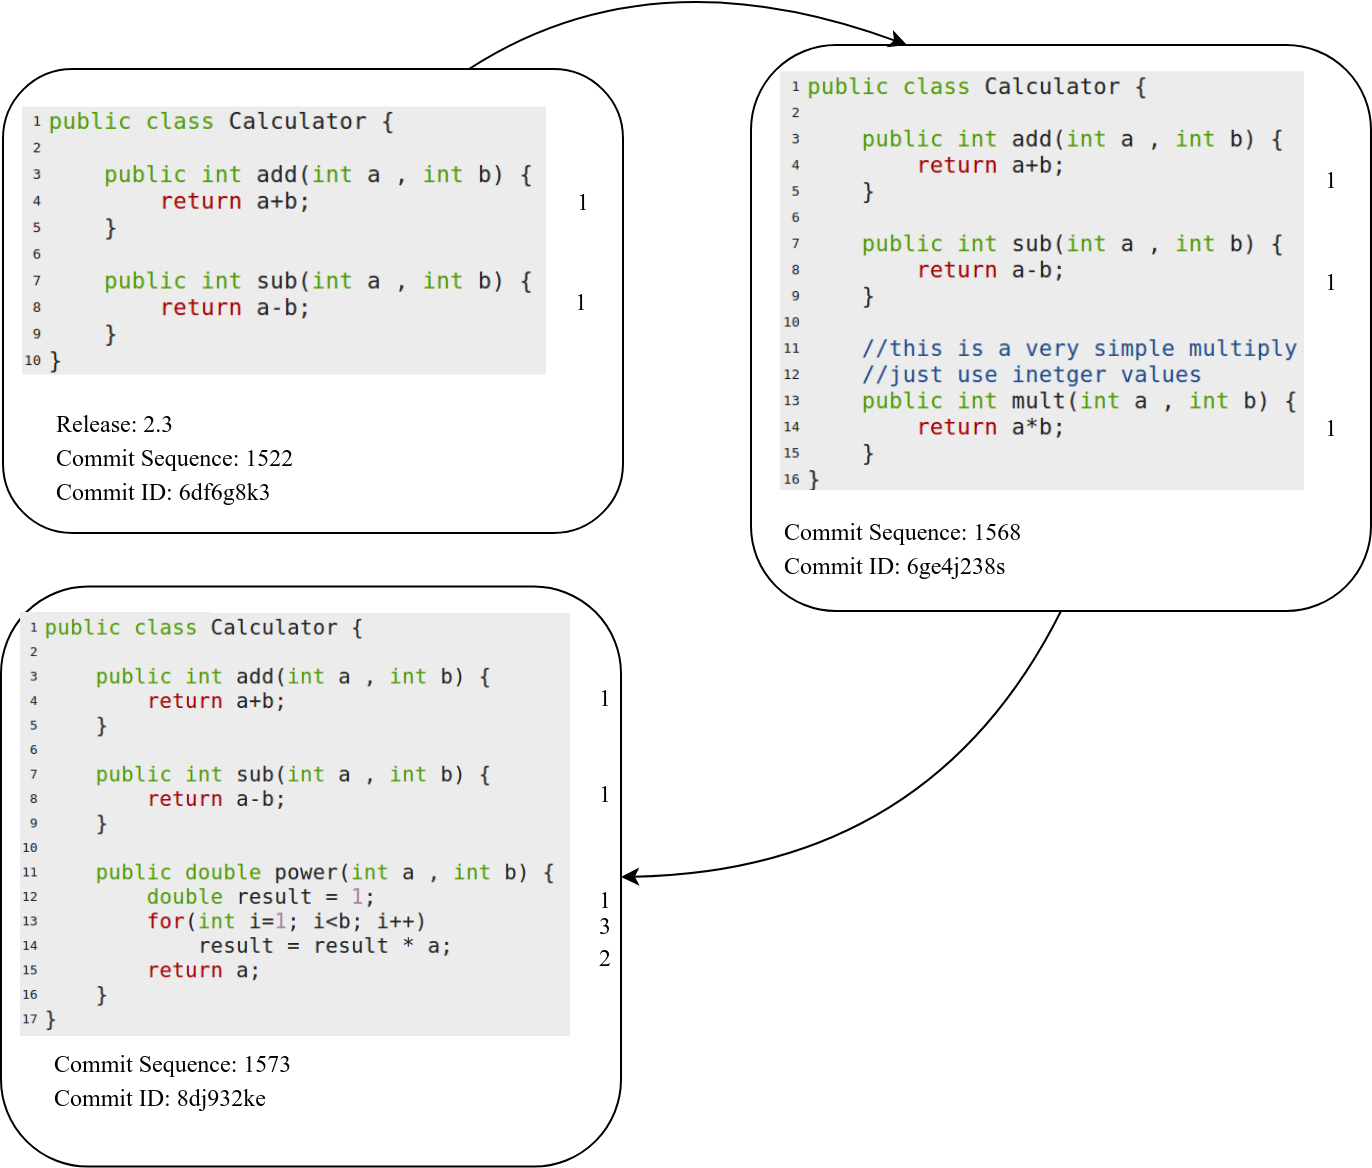
\includegraphics[width=1\textwidth]{img/method/example3.png}
	\caption{ تاریخچه‌ی پرونده‌یCalculator در مثال چهارم}
	\label{fig:example3}
\end{figure}

\section{JPredict}
جهت آگاهی از عملکرد معیارهای مطرح شده لازم است این معیارها استخراج شوند با استفاده از آنها مدل پیش‌بینی ساخته شود و با یکدیگر مقایسه شوند. جهت انجام این وظایف ابزار  در این پایانامه ابزار JPredict ارائه گردیده است که می‌تواند این وظایف را به صورت خودکار انجام دهد. همچنین قابلیت گسترش جهت کار با انواع مجموعه‌داده‌ها و استخراج معیارهای تعریف شده‌ی جدید توسط کاربر را دارد. 

نمای کلی از فرآیند‌هایی که در ابزار Jpredict انجام می‌گیرد در شکل \ref{fig:jpredict-process}  آمده است. این شکل نشان می‌دهد که در ابتدا انواع مختلفی از اطلاعات لازم است که از منابع متفاوت بدست آید. ابتدا اطلاعات پرونده‌های حاوی خطا از گزارش‌های خطا بیرون بدست می‌آید. این گزارش‌ها می‌توانند داده‌های موجود در سیستم ردگیری خطا و یا  مجموعه‌داده‌ی مرتبط با خطاهای پروژه‌های نرم‌افزاری باشد. همچنین تعدادی از پرونده‌های بدون نیز انتخاب می‌شوند. این انتخاب به صورت تصادفی انجام می‌شود و بسته به خواست کاربر محدودیت‌هایی در انتخاب در نظر گرفته می‌شود. اطلاعات این دو نوع پرونده با استفاده از سامانه‌ی کنترل نسخه تکمیل می‌گردد و در پایگاه داده ذخیره می‌شود. نوع دیگری از اطلاعات که از سامانه‌ی کنترل نسخه استخراج می‌شود اطلاعات تاریخی مربوط به توسعه‌ی پروژه‌ی نرم‌افزاری است. این اطلاعات بسته به معیارهایی که قرار است از آنها استخراج شود می‌تواند برای تمامی پرونده‌های موجود در سامانه‌ی کنترل نسخه استخراج شود و یا تنها برای پرونده‌های حاوی خطا و سالم انتخاب شده. معمولا در صورتی که استخراج اطلاعات پرهزینه باشد تنها برای پرونده‌های انتخابی اطلاعات تاریخی استخراج می‌شود. 

از آنجا که معیارهای جهش نیز باید محاسبه شوند لازم است تا برای پرونده‌های انتخابی کد منبع پروژه‌ی  مرتبط از سامانه‌ی کنترل نسخه بازیابی شود سپس با استفاده از یکی از ابزارهای جهش بر روی  پرونده تحلیل جهش انجام می‌گیرد. این دسته از اطلاعات  نیز در پایگاه‌داده ذخیره می‌شود. 

معیارهای مورد نظر با استفاده \واژه{پرسمان} مناسب از اطلاعات موجود در پایگاه داده استخراج می‌شوند و از آنها در ساخت مدل پیش‌بینی استفاده می‌گردد. مدل پیش‌بینی نمونه‌ی جدید را دریافت می‌کند و سالم یا خطادار بودن آنرا پیش‌بینی خواهد کرد. در واقع این نمونه یک بردار ویژگی از معیارهای استفاده شده در ساخت مدل است. در نهایت  با توجه به نتایج مدل ساخته شده ارزیابی می‌گردد.

\begin{figure}[H]
	\centering
	\includegraphics[width=1.0\textwidth]{img/method/jpredict-process.png}
	\caption{ نمایی کلی از فرآیند‌های موجود در JPredict}
	\label{fig:jpredict-process}
\end{figure}

\subsection{مزایای استفاده از روش Jpredict}
مزایای استفاده از روش پیشنهادی جهت استخراج معیارهای پیش‌بینی را می‌توان در موارد زیر خلاصه کرد. برخی از این موارد از مزایای عمومی استفاد از پایگاه داده می‌باشد که استخراج این معیارها بیشتر به چشم می‌خورند.
\begin{enumerate}
\item افزودن معیارهای جدید به معیارهای قابل استخراج به سهولت هرچه تمام‌تر و با کمترین هزینه انجام می‌گیرد

\item	

در صورت عدم ذخیره‌ی مناسب نتایج، هر بار ساخت اشیاء با اجرای برنامه بسیار زمانبر است و اتلاف وقت زیادی دارد. در این روش این مشکل حل شده است.
\item 
امکان از سرگیری محاسبات در صورت توقف به سادگی امکان پذیر است.

\item
لازم است برای اطمینان از درستی برنامه، داده‌ها در قالب جداولی به صورت چشمی کنترل شوند.
\item
فراخوانی و جستجو در پایگاه داده سریع است و کارایی بالا می‌رود.
\item
نگهداری از برنامه در دراز مدت راحت‌تر خواهد بود و خوانایی کدها بیشتر خواهد بود چرا که کار با پایگاه داده دارای اصول مشخصی است و سایرین از آن اطلاع دارند اما پرونده متنی اینگونه نیست.
\end{enumerate}

به عنوان مثال حالتی را در نظر بگیرید که  بدون استفاده از روش پیشنهادی  قرار است معیار تعداد ثبت‌ها محاسبه شود. در این حالت لازم است که به طور مستقیم جهت محاسبه با سیستم کنترل نسخه تعامل شود.  به این صورت که تعداد ثبت‌های بین ثبت کنونی و انتشار قبلی  را بررسی کرده و تعداد  ثبت‌هایی که در آن‌ها پرونده حاوی خطا تغییر کرده است شمرده شوند.\\ مشکل این راه این است که بسیار پر هزینه  خواهد بود زیرا مرتبا باید عملیات \واژه{ورودی/خروجی} بر روی دیسک انجام پذیرد و همچنین بررسی‌های تکراری بسیاری انجام می‌گیرد. به عنوان مثال دو ثبت حاوی خطا را در نظر بگیرید که دارای انتشار ما قبل یکسانی هستند. تعدادی از بررسی‌های ثبت‌های ما بین آن‌ها تا ثبت مربوط به انتشار دارای همپوشانی خواهد بود. از طرف دیگر می‌توان اطلاعاتی که در بررسی ثبت‌ها بدست می‌آید در محاسبه‌ی معیارهای دیگر نیز مورد استفاده قرار گیرد و هزینه‌های محاسباتی کاهش یابد. 

\subsection{ساختار Jpredict}
واحدهای اصلی تشکیل دهنده‌ی Jpredict در شکل \ref{fig:jpredict-module} نشان داده شده‌ است. واحد Mutation وظیفه‌ی تولید جهش و انجام تحلیل را بر عهده دارد و در واقع رابط میان Jpredict و ابزار  خارجی آزمون جهش می‌باشد. واحد Repository ارتباط با سامانه‌ی کنترل نسخه‌ی پروژه‌های مورد آزمایش را بر عهده دارند. اطلاعات لازم را بازیابی می‌کند و کد منبع ثبت‌های مختلف را در مسیری قرار می‌دهد تا ابزار جهش با آن کار کند. واحد BugReport اطلاعات پرونده‌های حاوی خطا را از منبع بیرونی دریافت می‌کند و با استفاده از واحد Repository آنها را تکمیل می‌کند.  انتخاب پرونده‌های سالم نیز بر عهده‌ی این واحد می‌باشد. واحد MutationMetric دستورات مرتب با جهش به واحد Mutation می‌دهد و نتایج اولیه را در پایگاه داده ذخیره می‌کند و با اجرای پرسمان مناسب معیارها را محاسبه می‌نماید. واحد ProcessMetric نیز  از داده‌هایی که واحد Reposiotry بر روی پایگاه داده ذخیره کرده است استفاده می‌کند و معیارهای فرآیند را محاسبه می‌کند. واحد DataBase وظیفه‌ی ارتباط با پایگاه داده‌ را دارد و همچنین حاوی پرسمان‌های مختلف است. در ادامه به بررسی جزیی‌تر هریک از واحدها پرداخته می‌شود.


\begin{figure}[H]
	\centering
	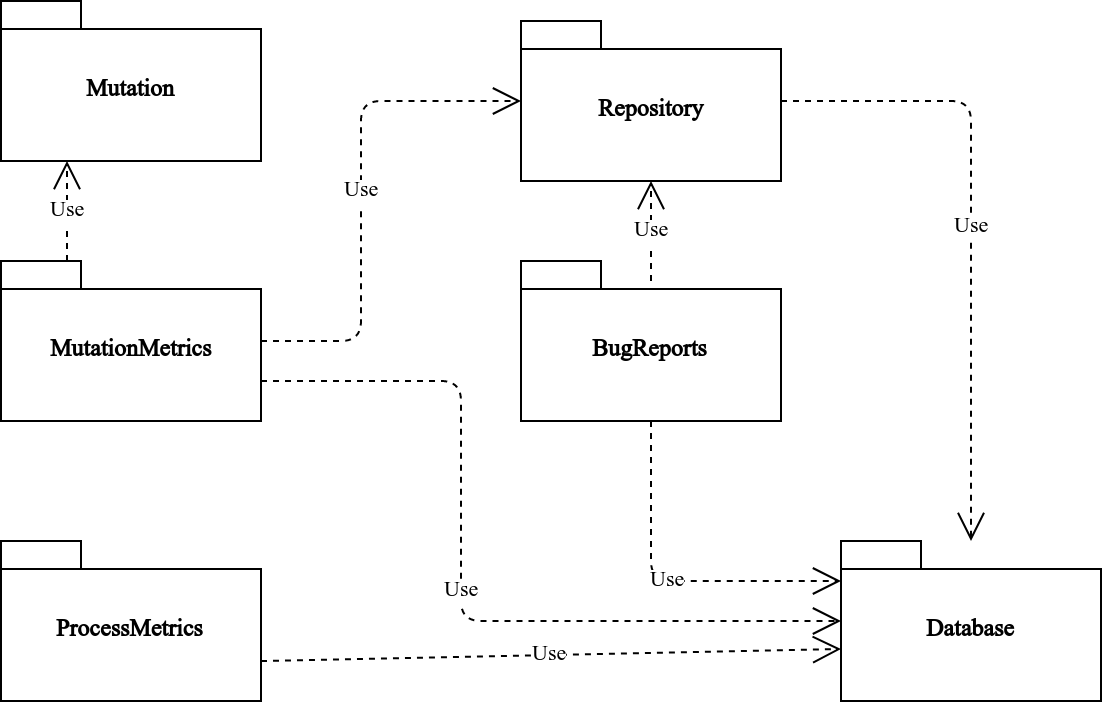
\includegraphics[width=.8\textwidth]{img/method/component-jpredict.png}
	\caption{ نمایی از واحدهای تشکیل دهنده‌ی JPredict}
	\label{fig:jpredict-module}
\end{figure}

\subsection{واحد  Repository}
 
همانطور که اشاره شد این واحد دو وظیفه‌ی اصلی دارد: استخراج اطلاعات از سامانه‌ی کنترل نسخه و دریافت کد منبع برای یک پروژه‌ی خاص. 

با توجه به مرور معیارهای استفاده شده در پژوهش‌های پیشین که در قسمت \ref{subsec:metrics}‌معرفی شدند و معیارهای انتخاب شده در قسمت \ref{sec:method-phase1}  لازم است اطلاعات زیر استخراج گردد.
\begin{itemize}
\item
اطلاعات ثبت‌های مختلف در پروژه شامل شماره‌ی ثبت در سامانه‌ی کنترل نسخه، نام ثبت‌کننده، پرونده‌های تغییر یافته در ثبت، تعداد خطوط حذف و اضافه شده
\item
انتشار قبلی ثبت‌ها
\item
مشارکت‌کنندگان در یک پرونده در زمان ثبت و میزان مشارکت آنها

\end{itemize}

پس از استخراج هر یک از این اطلاعات لازم است آنها به نحو مناسبی در پایگاه داده قرار گیرند. این واحد چهار جدول در پایگاه داده می‌سازد که در زیر مشخص شده‌اند:
\begin{itemize}
\item CommitInfo :
حاوی اطلاعات ثبت‌ها
\item CommitChangedFiles : 
حاوی اطلاعات پرونده‌های تغییر یافته در هر ثبت نسبت به ثبت قبلی
\item ProjectRelease :
انتشارهای موجود در پروژه‌ها
\item Participation :
مشارکت کنندگان در پرونده و میزان مشارکت آنها به تفکیک ثبت
\end{itemize}

وظیفه‌ی دیگر این واحد بازیابی کد منبع  پروژه در یک ثبت خاص  می‌باشد.  جهت انجام این امر،  برای هر سامانه‌ی کنترل نسخه لازم است از کتابخانه‌ی مناسب با آن کمک گرفته شود. یکی دیگر از وظایف این سامانه مشخص کردن تفاوت میان دو ثبت از پروژه است. از این قابلیت هم در مشخص کردن تعداد خطوط کم و اضافه شده در جدول CommitChangedFiles استفاده می‌شود و هم در محاسبه‌ی معیارهای ارائه شده‌ی جدید. 

\subsection{واحد ProcessMetrics}
معیارهای فرآیند در جدول متناظری ذخیره می‌شوند که  این جدول قبل از محاسبه‌ی معیارها مقداردهی اولیه می‌شود. هر سطر از این جدول به یکی از پرونده‌هایی که لازم است معیارها برای آن محاسبه شود اختصاص می‌یابد. این امر سبب می‌شود محاسبه‌ی هر معیار مستقل از دیگر انجام گیرد و امکان بروزرسانی داشته باشد. نحوه‌ی محاسبه‌ی یک معیار فرآیند در واحد ProcessMetrics در شکل \ref{fig:process-chart}  آمده است. در این فرآیند ابتدا اطلاعات پرونده‌ها از پایگاه داده بازیابی می‌گردد. سپس برای هر پرونده شئ مربوط به آن که حاوی معیارهای فرآیند است بازیابی می‌گردد. این شئ معادل یک سطر از جدول حاوی معیارهای فرآیند در پایگاه داده است. سپس لازم است که یک یا چند پرسمان تکمیل شود. این پرسمان‌ها از قبل در واحد Database  قرار دارند که نیازمند تکمیل هستند. پس از تکمیل آنها به واحد Database داده می‌شوند تا اجرا شوند. در صورت نیاز محاسبات بیشتری بر روی نتایج پرسمان انجام می‌گیرد. در نهایت شئ حاوی معیارهای فرآیند بروزرسانی می‌شود. 

به منظور محاسبه‌ی معیار فرآیند یک کلاس انتزاعی در نظر گرفته شده است که شامل مراحل نشان داده شده در شکل \ref{fig:process-chart}  است. هر معیار به طور جداگانه گسترشی از این کلاس خواهد بود که  قسمت‌های انتزاعی را پیاده‌سازی می‌کند. بدین ترتیب امکان افزودن معیار جدید فراهم می‌گردد. 
\begin{figure}[H]
	\centering
	\includegraphics[width=.8\textwidth]{img/method/process-chart.png}
	\caption{ فرآیند محاسبه‌ی یک معیار فرآیند در Jpredict}
	\label{fig:process-chart}
\end{figure}


\subsection{واحد BugReports  }
این واحد با منبع خارجی ارتباط برقرار می‌کند و اطلاعات پرونده‌های حاوی خطا را دریافت می‌کند. همچنین بر طبق محدودیت‌های از پیش تعیین شده تعدادی فایل سالم را از پروژه در یک ثبت خاص انتخاب کند. این انتخاب می‌تواند به صورت تصادفی انجام پذیرد و فایل‌های سالم نیز توسط منبع خارجی مشخص شود. سپس به کمک واحد Repository اطلاعات پرونده تکمیل می‌گردد و در پایگاه داده ذخیره می‌شود. اطلاعات مربوط به پرونده‌های حاوی خطا در جدول BugInfo و پرونده‌های سالم در جدول CleanInfo  قرار می‌گیرد. اطلاعاتی که در این دو جدول وجود دارد عبارتند از :
\begin{itemize}
	\item 
	نام پرونده‌ی حاوی خطا
	\item
	شماره‌ی خطا (در صورتی که یک خطا بیش از چند پرونده را شامل می‌شود)
	\item
	شماره‌ی ثبتی که در آن در پرونده‌ی مورد نظر خطا رخ داده
	\item
	نام انتشار قبلی
	\item
	شماره‌ی ثبت انتشار قبلی
	\item 
	نام پروژه (در حالتی که اطلاعات خطای چندید پروژه‌ی مختلف وجود دارد)
\end{itemize}

\subsection{واحد Mutation}
این واحد ارتباط میان Jpredict و ابزار جهش را برقرار می‌سازد. فرآیندهایی که در این واحد انجام می‌شوند در شکل \ref{fig:mutation-chart} آمده است. محل پرونده‌ی مورد نظر توسط واحد MutationMetric به این واحد داده می‌شود. این محل شامل سایر پرونده‌های پروژه نیز می‌شود. سپس پروژه آماده می‌گردد. این آماده‌سازی به این جهت است که ابزارهای جهش اغلب نیازمند آن هستند که پروژه کامپایل شود و برای  کامپایل صحیح آنها لازم است که پیکربندی‌هایی انجام شود و یا وابستگی‌های پروژه اضافه شود. پس از آماده سازی جهش‌یافته‌ها برای پرونده‌ی مورد نظر ساخته می‌شوند. سپس در صورت لزوم تحلیل جهش انجام می‌گردد. ممکن است به تحلیل جهش نیازی نباشد چراکه برخی معیارها تنها با تولید جهش یافته محاسبه می‌گردد. در پایان باید گزارش از ابزار جهش دریافت شود و به شکل مناسب جهت استفاده در واحد MutationMetric در بیاید. 

به منظور انجام این فرآیندها یک کلاس انتزاعی در نظر گرفته شده است که شامل مراحل نشان داده شده در شکل \ref{fig:mutation-chart}  است. برای انجام عملیات جهش بر روی هر پروژه می‌توان این کلاس را گسترش داد تا آماده‌سازی‌ها متناسب با آن پروژه پیاده‌سازی شود. بدین ترتیب امکان انجام جهش بر روی پروژه‌های جدید فراهم می‌گردد.

\begin{figure}[H]
	\centering
	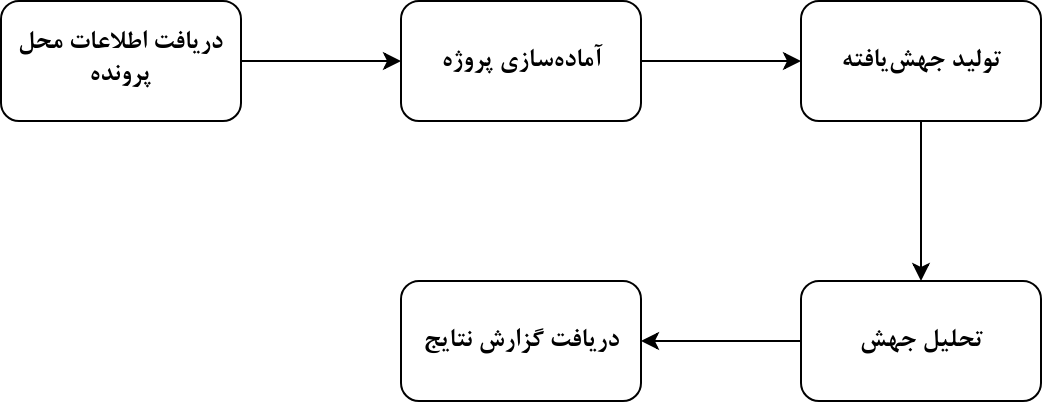
\includegraphics[width=.8\textwidth]{img/method/mutation-chart.png}
	\caption{ فرآیند‌های واحد Mutation}
	\label{fig:mutation-chart}
\end{figure}

\subsection{واحد MutationMetrics}

معیارهایی که به وسیله‌ی جهش به دست می‌آیند مشابه معیارهای فرآیند در جدول متناظری ذخیره می‌شوند که  این جدول قبل از محاسبه‌ی معیارها مقداردهی اولیه می‌شود. هر سطر از این جدول به یکی از پرونده‌هایی که لازم است معیارها برای آن محاسبه شود اختصاص می‌یابد.  نحوه‌ی محاسبه‌ی یک معیار بر اساس جهش در شکل \ref{fig:mutationmetircs-chart} آمده است. در این فرآیند ابتدا اطلاعات پرونده‌ها از پایگاه داده بازیابی می‌گردد. سپس برای هر پرونده شئ مربوط به آن که حاوی معیارهای  مبتنی  بر جهش است بازیابی می‌گردد. با استفاده از واحد Repository‌ پرونده‌های ثبت مورد نظر بازیابی می‌شود. سپس با استفاده از واحد Mutation عملیات جهش انجام می‌گیرد. در محاسبه‌ی معیارهای جهش نیاز به سایر ثبت‌های پرونده نیست. در دو دسته‌ی دیگر لازم است که سایر ثبت‌ها نیز بازیابی شود و عملیات جهش بر روی آنها نیز انجام شود در این صورت نتایج میانی در پایگاه داده ذخیره می‌شود.  در حالتی که نتایج میانی وجود دارد، محاسبات اضافی انجام خواهد گرفت.  در نهایت معیار محاسبه شده در شئ حاوی معیارها قرار می‌گیرد. 

 داده‌هایی که برای محاسبه‌ی معیارهای جدید ارائه شده لازم است محاسبه شود در زیر آمده است. همچنین جدولی که داده‌ها در آن قرار می‌گیرد مشخص شده است.
\begin{itemize}
	\item
	تعداد جهش‌یافته‌های جدید برای یک پرونده در ثبت مورد نظر نسبت به آخرین انتشار قبلی: این معیار نتایج میانی ندارد و پس از محاسبات مستقیما در کنار سایر معیارهای مبتنی بر جهش قرار می‌گیرد. 

\item 
تعداد جهش‌یافته‌های جدید برای یک پرونده در یک انتشار نسبت به 
انتشار قبلی: این داده‌ها در جدولی به نام DistinctMutantLog قرار می‌گیرد.

\item 
تعداد جهش‌یافته‌های اضافه و کم شده برای یک پرونده در یک ثبت نسبت به ثبت قبلی: داده‌ها در جدول MutantsChange قرار می‌گیرد.

\item
تغییرات امتیاز جهش برای یک پرونده در یک انتشار نسبت به انتشار قبلی: داده‌ها در جدول  ReleaseMutation قرار می‌گیرد. 

\end{itemize}

\begin{figure}[H]
	\centering
	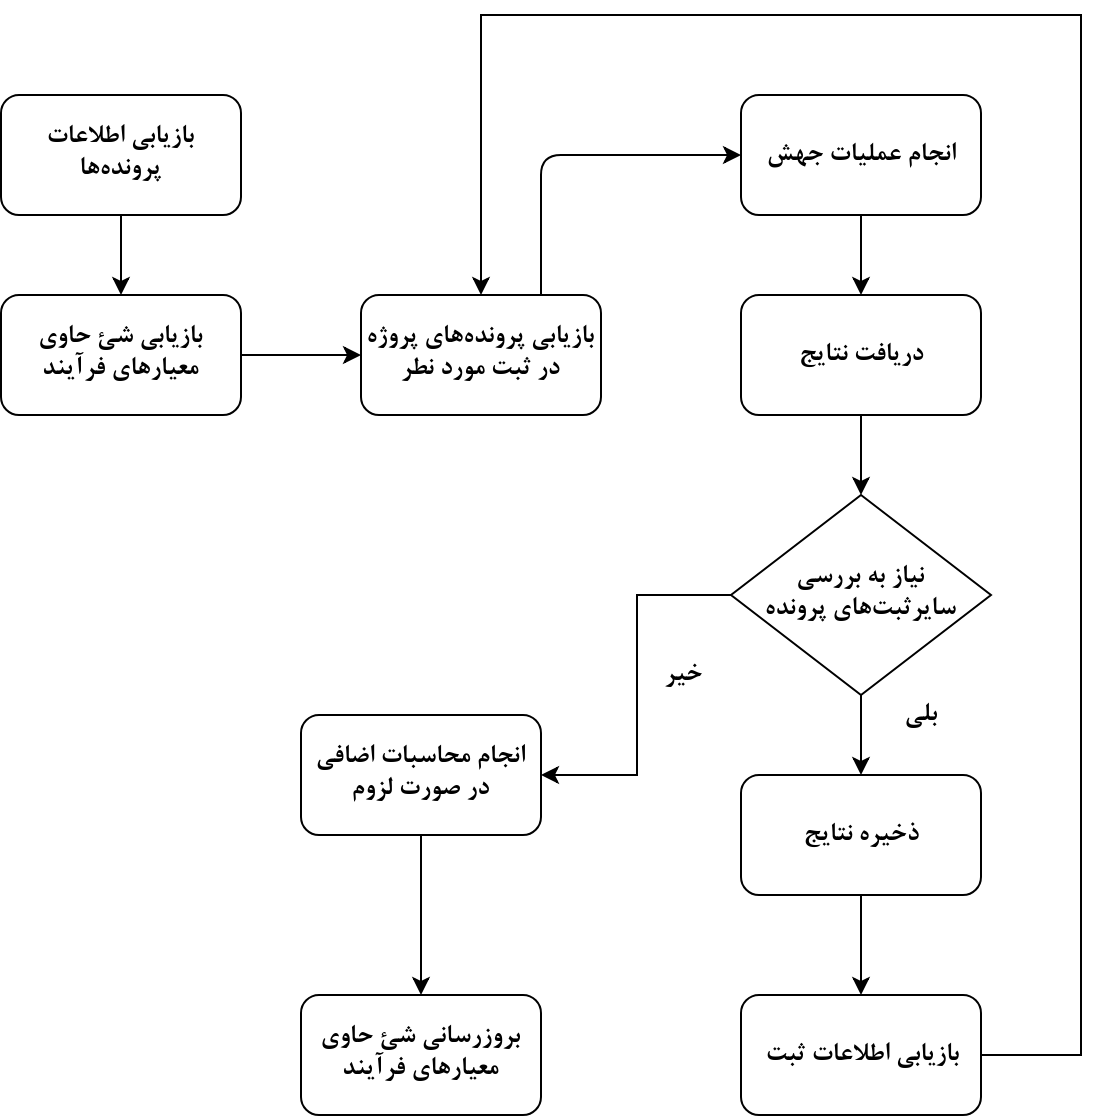
\includegraphics[width=.7\textwidth]{img/method/MutationMetrics-Chart.png}
	\caption{ فرآیند‌های واحد MutationMetrics}
	\label{fig:mutationmetircs-chart}
\end{figure}

\subsection{واحد Database}

همانطور که بیان شد این واحد ارتباط میان پایگاه‌داده و JPredict را برقرار می‌کند. در این واحد یک کلاس انتزاعی به منظور دسترسی به جداول قرار داده شده است.  برای هر جدول یک گسترش از کلاس انتزاعی ساخته می‌شود  به نمونه‌های این کلاس‌ها، شئ دسترسی به داده  گفته می‌شود. پرسمان‌های مربوط به هر جدول  نیز از طریق کلاس متناظر اجرا می‌گردد. نمودار EER جداول ساخته شده در شکل \ref{fig:EER} آمده است.
\begin{figure}[H]
	\centering
	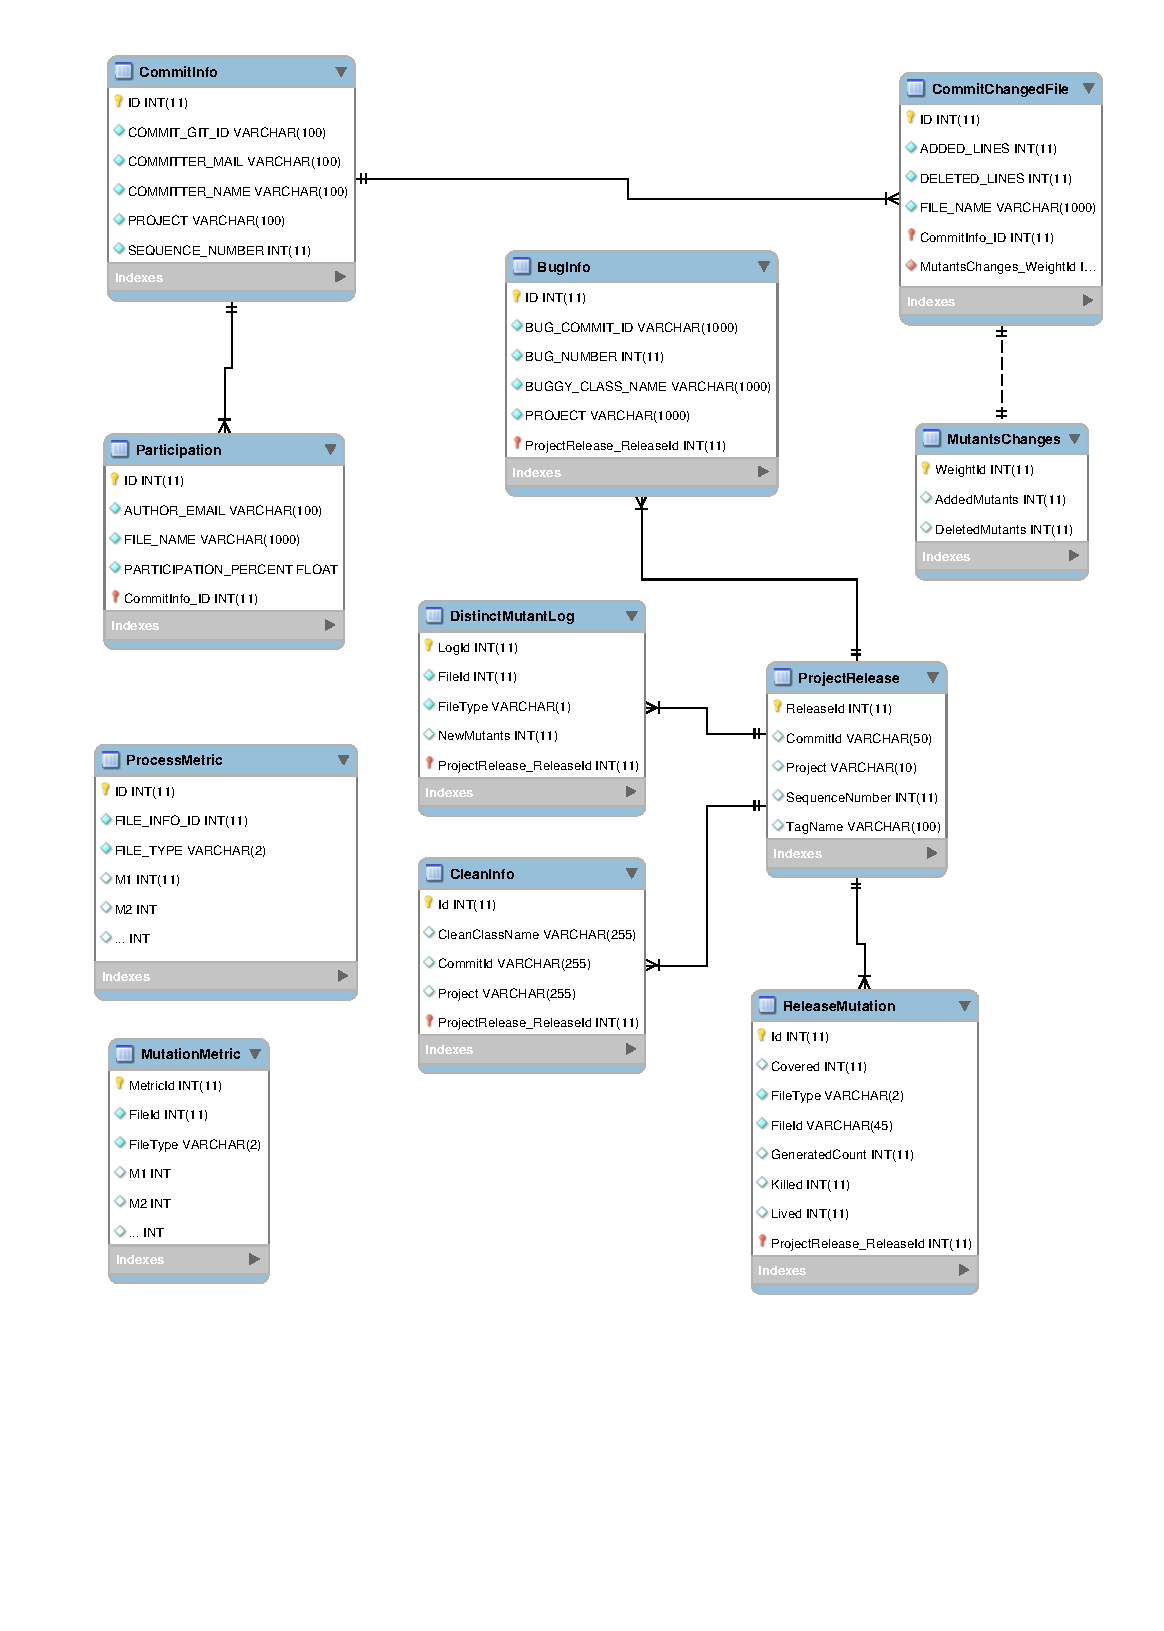
\includegraphics[trim={0 5cm 0 0},width=1\textwidth]{img/method/EER.pdf}
	\caption{ نمودار EER جداول ساخته شده}
	\label{fig:EER}
\end{figure}

\subsection{محاسبه‌ی معیارها در روش پیشنهادی}

محاسبه‌ی معیارهای مطرح شده با استفاده از روش پیشنهادی به طور کلی به این صورت است که پرسمان‌هایی طراحی می‌شود تا به وسیله‌ی آنها معیارها محاسبه شود. در قسمت زیر پرسمان‌های لازم  برای هر معیار آورده شده است. این پرسمان‌ها را می‌توان متناسب با هر نوع پایگاه داده پیاده‌سازی نمود. لازم به ذکر است که در صورتی که از جدوال برای نگهداری اطلاعات چندین پروژه‌ی مختلف استفاده  شود لازم است شرط تعلق به پروژه‌ی مورد نظر به پرسمان‌های زیر افزوده شود.  در این پرسمان‌ها به منظور تمایز و شناسایی افراد از ایمیل‌ آنها می‌توان استفاده کرد.   امکان استفاده از هر شناساگر دیگر که بتوان به وسیله‌ی آن افراد را شناسایی و متمایز کرد وجود دارد. البته این شناساگر باید در تمام جداول یکسان باشد. 
\begin{itemize}
	\item 
	تعداد ثبت:  تعداد سطر‌های جدول CommitChangedFile که نام آنها برابر پرونده‌ی مورد نظر است و ثبت متناظر با آن سطر در بازه‌ی انتشار قبلی تا ثبت مورد نظر پرونده قرار دارد.
	
	\item 
	تعداد توسعه‌دهندگان فعال:  تعداد متمایز ثبت‌کننده‌گان از جدول CommitInfo که ثبت متناظر با آن در بازه‌ی آخرین انتشار و ثبت مورد نظر است. همچنین  شناسه‌ی ثبت در بین شناسه‌هایی از جدول CommitChangedFile باشد که برای آن شناسه‌ی ثبت فایل مورد نظر تغییر کرده است.
	\item
	تعداد توسعه‌دهندگان متمایز: تعداد متمایز ثبت‌کننده‌گان از جدول CommitInfo که ثبت متناظر با آن در بازه‌ی  اولین ثبت از پروژه تا ثبت مورد نظر است. همچنین  شناسه‌ی ثبت در بین شناسه‌هایی از جدول CommitChangedFile باشد که برای آن شناسه‌ی ثبت فایل مورد نظر تغییر کرده است.  
	\item
	مقدار نرمال‌سازی شده‌ی تعداد خطوط اضافه شده: برای این معیار لازم است از دو پرسمان استفاده شود. پرسمان اول مجموع خطوط اضافه شده در پرونده را می‌شمارد و پرسمان دوم مجموع خطوط اضافه شده در پروژه را می‌شمارد.\\
	پرسمان اول: مجموع خطوط اضافه شده در سطرهایی از جدول CommitChangedInfo که ثبت متناظر با آنها در بازه‌ی آخرین انتشار و ثبت مورد نظر است و همچنین آن سطر متعلق به پرونده‌ی مورد نظر می‌باشد. 
	پرسمان دوم: مجموع خطوط اضافه شده در سطرهایی از جدول CommitChangedInfo که ثبت متناظر با آنها در بازه‌ی آخرین انتشار و ثبت مورد نظر است.\\
	به منظور محاسبه معیار پرسمان اول بر دوم تقسیم می‌گردد. 
\item
مقدار نرمال‌سازی شده‌ی تعداد خطوط اضافه شده: مشابه معیار قبل با این تفاوت که مجموع خطوط حذف شده در نظر گرفته می‌شود. 
\item
درصد خطوطی که مالک پرونده مشارکت کرده: مقدار حداکثر از میان سطرهای جدول Participation که متعلق به پرونده‌ی مورد نظر در ثبت مورد نظر است. 
\item 
تعداد مشارکت‌کنندگان جزیی: تعداد ایمیل‌های نویسندگان در جدول Participation در سطرهایی که متعلق به پرونده‌ی مورد نظر در ثبت مورد نظر است و میزان مشارکت آنها کمتر از ۵ درصد است. 
\item
تعداد ثبت‌های همسایگان: برای این معیار دو پرسمان لازم است. پرسمان اول همسایگان و تعداد همسایگی پیدا می‌کند. پرسمان دوم تعداد ثبت‌ها را می‌شمارد که درباره‌ی آن توضیح داده شد. \\
پرسمان اول: سطرهایی از جدول CommitChangedFile که ثبت متناظر در میان ثبت‌هایی است که در آنها فایل مورد نظر تغییر کرده و آن ثبت در بازه‌ی انتشار قبلی تا ثبت مورد نظر انجام شده. همچنین آن سطر نباید متعلق به پرونده‌ی مورد نظر باشد. سطر‌های انتخاب شده باید بر اساس نام پرونده‌ی آنها گروهبندی شود و در این گروه‌بندی تعداد سطر‌ها در هر گروه مشخص شود. 
\item
تعداد توسعه‌دهندگان فعال همسایگان: مشابه معیار قبل با این تفاوت که در پرسمان دوم معیار توسعه‌دهنگان فعال محاسبه می‌شود.
\item
تعداد توسعه‌دهندگان متمایز همسایگان: مشابه معیار قبل با این تفاوت که در پرسمان دوم معیار توسعه‌دهنگان متمایز محاسبه می‌شود.
\item
تجربه‌ی مالک پرونده: این معیار به دو پرسمان نیاز دارد. یک پرسمان جهت یافتن مالک پرونده و پرسمان دیگر تعداد ثبت‌های فرد یافت شده در پروژه را می‌شمارد. \\
پرسمان اول: فردی که در جدول Participation میزان مشارکت وی در پرونده در ثبت مورد نظر برابر بیشترین میزان مشارکت در بین سطرهای متعلق به آن پرونده در آن سطر است.\\
پرسمان دوم: تعداد ثبت‌هایی که توسط فرد مشخص شده در پرسمان اول در بازه‌ی آخرین انتشار و  ثبت مورد نظر انجام شده است. 
\item
تجربه‌ی تمام توسعه‌دهندگان: این معیار دو پرسمان احتیاج دارد. پرسمان اول لیست تمام توسعه‌دهندگان را پیدا می‌کند و پرسمان دوم برای هر فرد تجربه‌ی وی را استخراج می‌کند که برابر پرسمان دوم معیار قبلی است. 
\item

\end{itemize}
 
اکثر معیارهای مبتنی بر جهش به پرسمان خاصی جهت محاسبه نیاز ندارند و بیشتر پرسمان‌ها جهت بازیابی اطلاعات پرونده‌ها و نتایج میانی است. دو پرسمان پرکاربرد در زیر آمده‌اند. علت ایجاد جداول اضافی در محاسبه‌ی  این معیارها پایداری در انجام محاسبات است.  به علت زمان‌بر بودن عملیات جهش  در صورت توقف محاسبات امکان از سرگیری محاسبات از محل توقف وجود  دارد و همچنین  با نگهداری به عنوان یک مجموعه داده می‌تواند در پژوهش‌های دیگر به کار گرفته شود. همچنین مزایای عمومی استفاده از پایگاه داده در محاسبه‌ی معیارها در مورد این دسته نیز صادق است. 

\begin{itemize}
\item
	 چهار انتشار اخیر یک ثبت: از جدول ProjectRelease انتشارهایی از پروژه انتخاب می‌شوند و شماره‌ی دنباله‌ی آنها از شماره‌ دنباله‌ی انتشار قبلی ثبت مورد نظر کمتر است. این سطر‌ها بر اساس  شماره‌ی دنباله نزولی مرتب می‌شوند و چهار انتشار برتر انتخاب می‌شوند. 
\item
ثبت‌هایی که در آنها پرونده‌ی مورد نظر تغییر کرده: ثبت‌هایی از جدول CommitInfo انتخاب می‌شوند که در بازه‌ی انتشار قبلی تا ثبت کنونی انجام شده‌اند و در جدول CommitChangedFile سطری برای آن ثبت وجود داشته باشد که نشان دهد در آن پرونده‌ی مورد نظر تغییر کرده است. همچنین ثبت‌های انتخاب شده باید بر اساس شماره‌ی دنباله مرتب شوند. 
	 
\end{itemize}





